% https://github.com/tribler/Tribler/wiki
% https://github.com/Tribler/tribler/wiki/Anonymous-Downloading-and-Streaming-specifications
% Screenshots voor tribler anonymous tunnels

\section{Tribler}
	\label{sec:tribler}
	In this section an overview of Tribler and its components is presented. We describe the new trial version that uses anonymous tunnels in depth. Furthermore, we look at what specific dependencies Tribler relies on.

	Tribler is a fully decentralized peer-to-peer file sharing system developed by the Parallel and Distributed Systems group at Delft University of Technology. It has been in development for over nine years and has a mature and well-established code base. It allows users to search for and share files in a fully decentralized way. The decentralized nature of Tribler has several advantages over existing file sharing systems. The lack of a centralized component makes it scalable and practically impossible to bring down. 

	An experimental version of Tribler is currently available that includes a Python implementation of a Tor-like protocol. This enables users to share files anonymously. By encrypting and routing traffic over a circuit of nodes, it ensures the communicating parties are oblivious of each other's virtual and physical location.
	
	\subsection{Downloading files}
		Tribler uses the torrent protocol\footnote{\href{http://www.bittorrent.org/beps/bep\_0003.html}{www.bittorrent.org/beps/bep\_0003.html}} for downloading files. Torrent files contain metadata about the files that will be downloaded. The torrent protocol is peer-to-peer, which means that users download from each other. Users that provide files for their peers are called seeders. Tribler is using the libtorrent library as an implementation of the torrent protocol. This library is licensed as open source software and we are allowed to use or modify it.
		
		Torrent files can be found using the graphical user interface (GUI) of Tribler. Users enter their search query in a search bar and Tribler will return the results matching the search criteria. A family filter has been added to Tribler to filter out adult content. The underlying search is done using Dispersy which will be described in Subsection \ref{sec:dispersy}. In Figure \ref{fig:tribleroverview} a general overview of the download process is given. The individual components like Dispersy and the anontunnels are described in more detail in the following sections.
		
		\begin{figure*}[!htb]
			\centering
			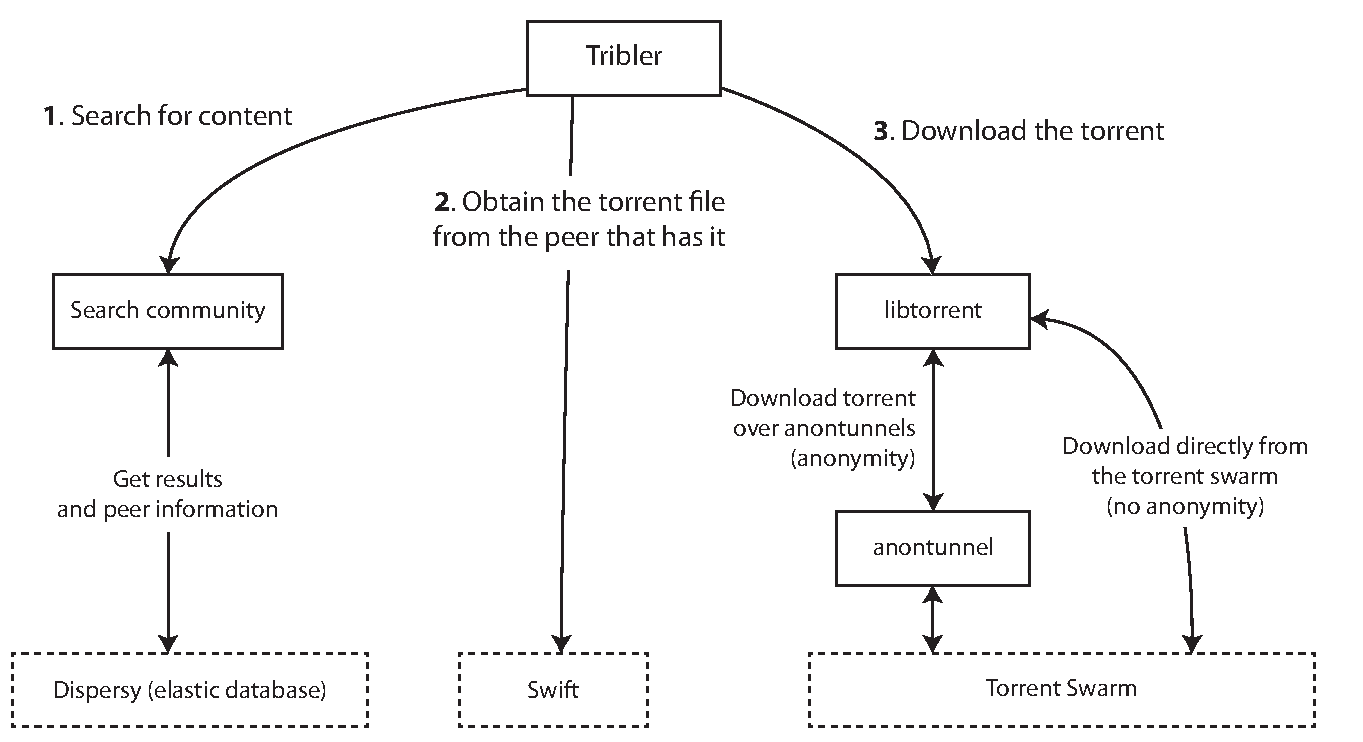
\includegraphics[width=\textwidth]{graphics/tribler-overview.pdf}
			\caption{An overview of downloading a file using Tribler.}
			\label{fig:tribleroverview}
		\end{figure*}
	
	\subsection{Anonymous tunnels}
		\label{sec:anonymoustunnels}
			Recently, the research team of Tribler started to work on the implementation of anonymous downloads. Pull request\footnote{\href{http://oss-watch.ac.uk/resources/pullrequest}{oss-watch.ac.uk/resources/pullrequest}} 525 on the Tribler GitHub page \cite{pullrequest525} is an experimental build of Tribler with the implementation of anonymous communications. The anonymous communication is achieved by using a Tor-like protocol. This protocol uses a three-hop circuit for anonymous communication. A circuit is a route from source to destination running over relay nodes (also called hops). Three-hop means that data travels over three nodes before it reaches the destination, to add anonymity. Note that Tribler does not use the Tor network, only a Tor-like protocol with UDP connections\footnote{\href{http://www.erg.abdn.ac.uk/~gorry/eg3561/inet-pages/udp.html}{www.erg.abdn.ac.uk/~gorry/eg3561/inet-pages/udp.html}}.
			
			The Python module \texttt{Tribler.community.anontunnel}\footnote{\href{https://github.com/Tribler/tribler/tree/devel/Tribler/community/anontunnel}{www.github.com/Tribler/tribler/tree/devel/Tribler/community/anontunnel}} contains the implementation of the anonymous tunnels.. Taking the code as reference, we now describe various details of the anonymous tunnels.
			
			\begin{itemize} 
				\item The circuit setup is using the Diffie-Hellman\footnote{\href{http://www.ietf.org/rfc/rfc2631.txt}{www.ietf.org/rfc/rfc2631.txt}} key exchange protocol to establish a secure connection. The M2Crypto library which is explained in Subsection \ref{sec:security}, performs the Diffie-Hellman key exchange.
				\item The experimental code is using the Socks5\footnote{\href{http://www.ietf.org/rfc/rfc1928.txt}{www.ietf.org/rfc/rfc1928.txt}} protocol for communication (see Figure \ref{fig:onion_encryption_decryption_socks5}).
				\item Dispersy is used as a data synchronization system. 
			\end{itemize}
			
			In order to test the anonymous connections and the download speed, a special anonymous tab has been built into Tribler. Clicking on this tab brings up a graph of the current anonymous network as a graph (see Figure \ref{fig:anon_downloads}). It also logs the circuit events such as when extending or creating a circuit. When enough nodes are online, a 50 MB test download file starts to download.
			
			\begin{figure*}[!htb]
				\centering
				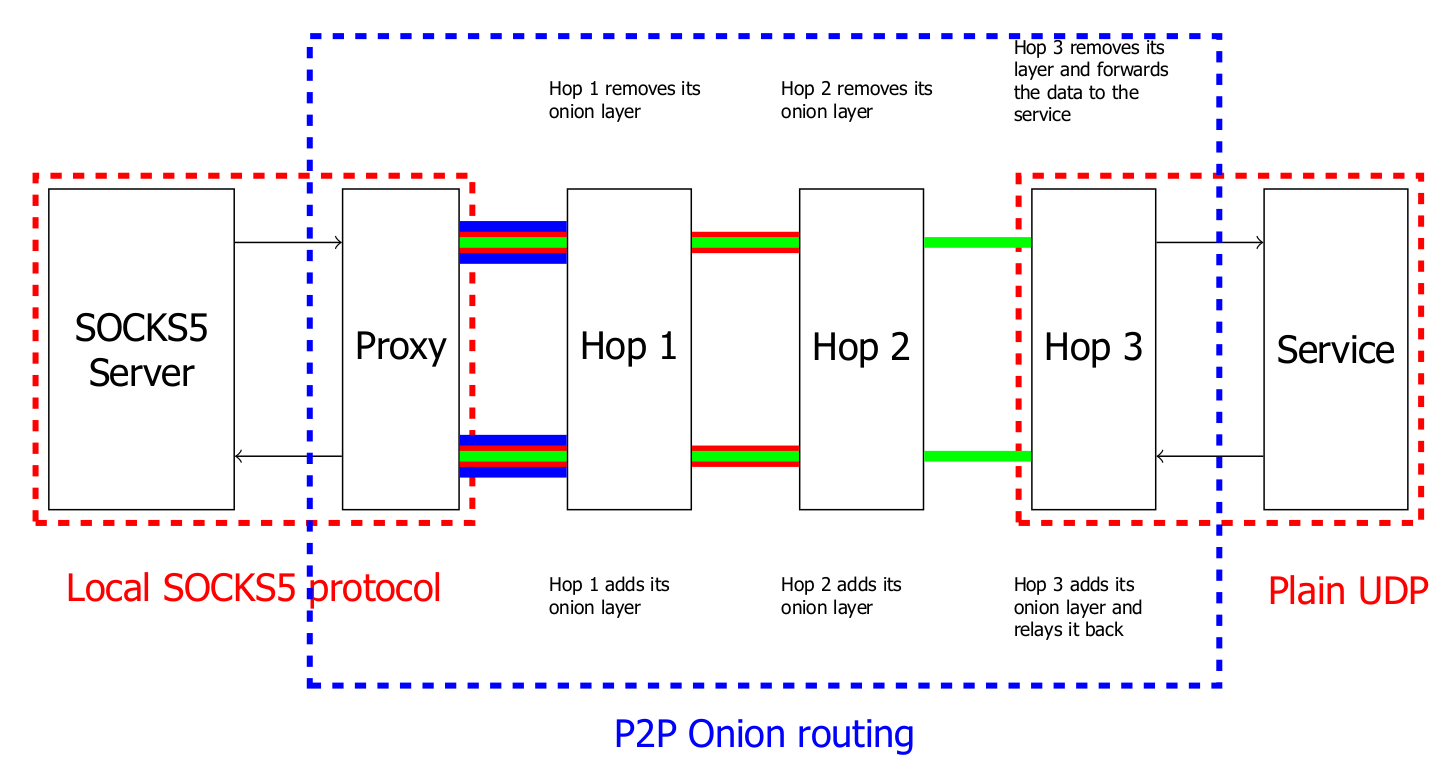
\includegraphics[width=\textwidth]{graphics/onion_encryption_decryption_socks5.png}
				\caption{The onion encryption and decryption used by the anontunnels. Taken from \href{https://github.com/Tribler/tribler/wiki/Anonymous-Downloading-and-Streaming-specifications}{www.github.com/Tribler/tribler/wiki/Anonymous-Downloading-and-Streaming-specifications}}
				\label{fig:onion_encryption_decryption_socks5}
			\end{figure*}

	\subsection{Security}
	\label{sec:security}
		Tribler makes use of cryptographic functions to encrypt data and make secure communication possible. Security is a big issue in the world of peer-to-peer networks. Not only do we want anonymous downloads, we also want confidentiality and integrity of our data. Confidentiality means that unauthorized parties cannot see the content of the information. This could be achieved by encrypting the data. Integrity of the data means that the data is protected from being modified by other parties or the network. Integrity is important when verification of the data is required.
		
		Some well-known open source frameworks exist for these cryptographic tasks. An example is OpenSSL \cite{openssl}. OpenSSL implements the popular SSL and TLS protocols\footnote{\href{http://tools.ietf.org/html/rfc5246}{tools.ietf.org/html/rfc5246}}. These are cryptographic protocols that provide security when communicating over the internet. Besides that, OpenSSL provides libraries for various encryption and decryption protocols such as 3DES\footnote{\href{http://tools.ietf.org/html/rfc2420}{tools.ietf.org/html/rfc2420}}, RSA\footnote{\href{http://www.ietf.org/rfc/rfc2437.txt}{www.ietf.org/rfc/rfc2437.txt}} and RC4\footnote{\href{http://tools.ietf.org/html/rfc4757}{tools.ietf.org/html/rfc4757}}. OpenSSL also supports key exchange protocols such as Diffie-Hellman\footnote{\href{http://www.ietf.org/rfc/rfc2631.txt}{www.ietf.org/rfc/rfc2631.txt}}.
		
		OpenSSL is written in the C programming language. To use the OpenSSL libraries in Python, Tribler uses M2Crypto \cite{m2cryptogithub}. The M2Crypto library, which acts a wrapper for OpenSSL, provides many implementations of popular cryptographic protocols that are used for secure communication.
		
	\subsection{Dispersy}
	\label{sec:dispersy}
		Tribler makes use of Dispersy. As elaborated by Zeilemaker et al; Dispersy \cite{zeilemaker2013dispersy} is a fully decentralized system for data bundle synchronization. This means that data is exchanged between peers to make sure they are up-to-date with the same information. The system is designed in such a way that it is capable of running in a challenging network environment. Such an environment is often characterized by:
		\begin{itemize}
			\item Nodes randomly joining and leaving.
			\item Delays in the network.
			\item Nodes having different networking speeds (Edge, 3G, WiFi).
			\item Nodes often being behind routers that use Network Address Translating (NAT) and firewalls.
		\end{itemize}
		
		All communication done by Dispersy uses UDP. Because up to 64\% of the Internet is behind a NAT, Dispersy has to use UDP NAT-firewall puncturing mechanisms\cite{zeilemaker2013dispersy}.
		
		In Dispersy, each node has a candidate list. A candidate list is a list of active connections within the node's overlay. Using this candidate list, a node can exchange data with its peers.
		
		\begin{figure*}[!t]
			\centering
			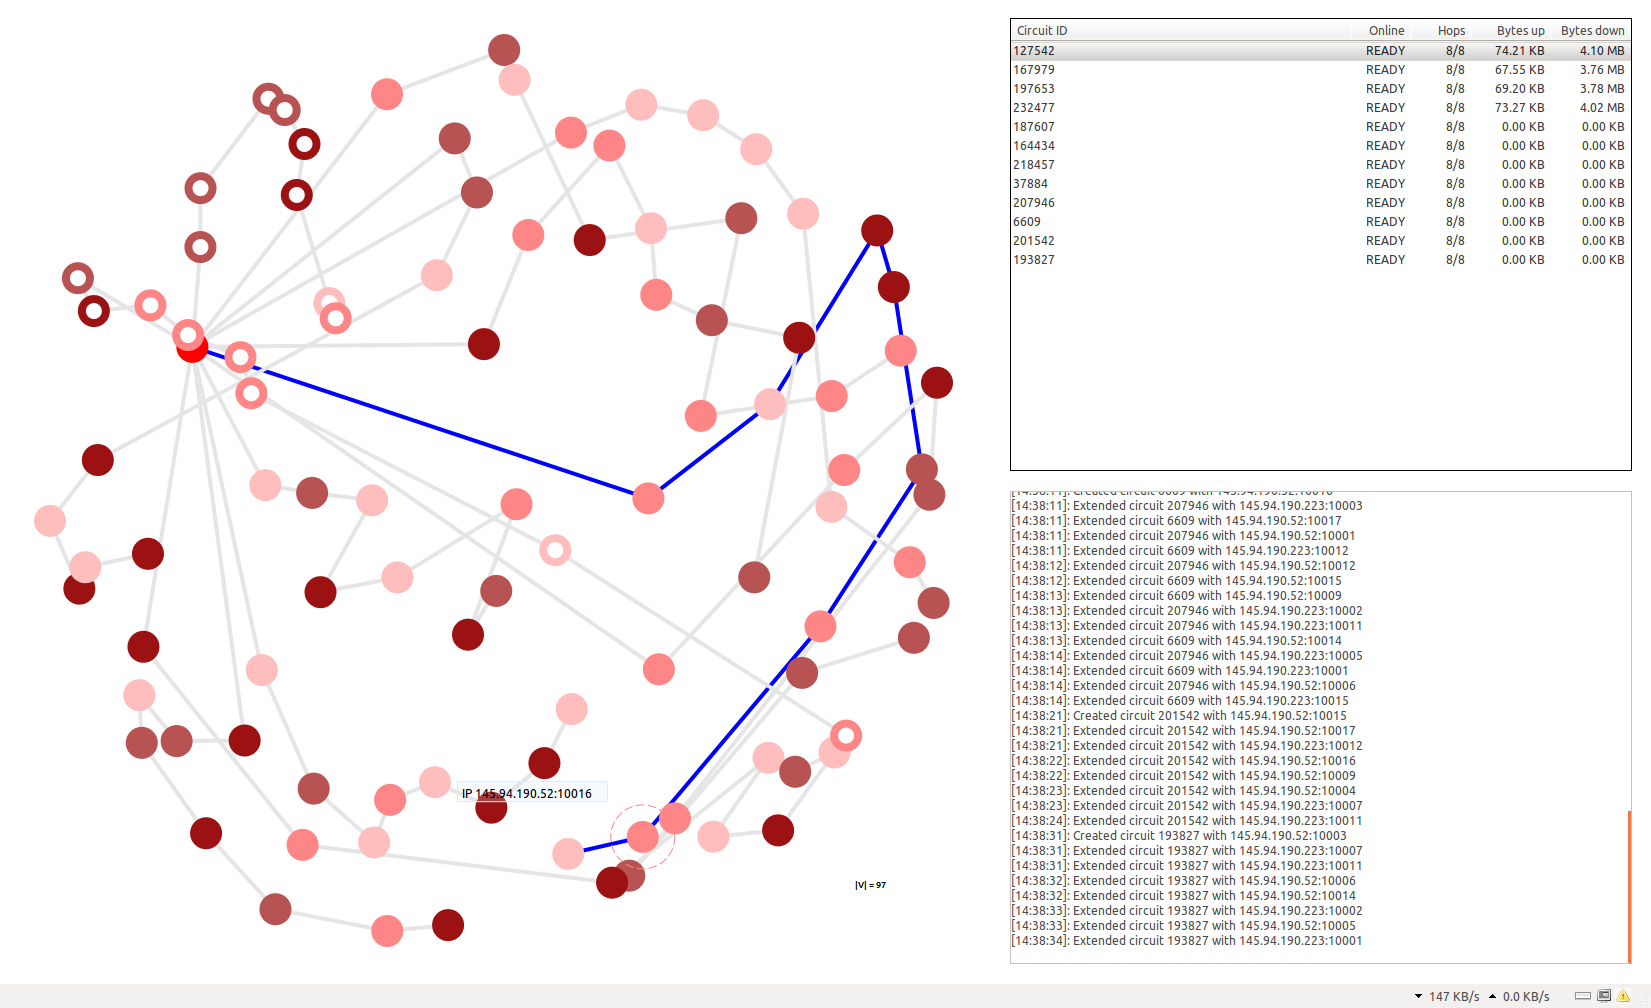
\includegraphics[width=0.8\textwidth]{prior-work/8hop.png}
			\caption{The graphical user interface in Tribler that shows the anonymous network.}
			\label{fig:anon_downloads}
		\end{figure*}